%
% mean.tex -- 
%
% (c) 2019 Prof Dr Andreas Mueller
%
\section{The mean value property of harmonic functions}
\rhead{Mean value property}
Harmonic functions have a property that is even stronger than
the maximum principle for elliptic operators.
The maximum principle says that the solution of a homogeneous elliptic
partial differential equation is bounded above and below by the
extreme values on the boundary.
The mean value property in addition says that the value in some
point is actually the mean of all the values in small circle
around the point.

\subsection{Mean value property}
In this section we are going to illustrate that the values of harmonic
functions are means of the values of the function on a sphere around 
the point.
\begin{figure}
\centering
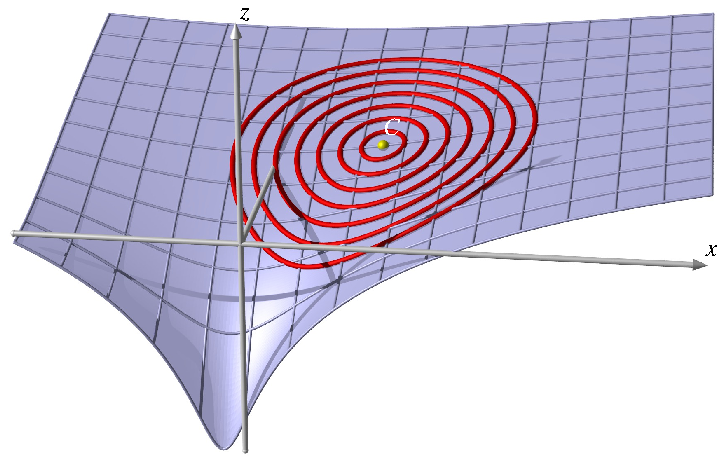
\includegraphics{7-elliptic/images/meanvalue.pdf}
\caption{Mean value property of a harmonic function.
The surface represents a harmonic function. 
The mean value along each of the red circles gives the same value,
namely the function value in the yellow center point $C$.
\label{elliptic:meanvalue:image}}
\end{figure}

\begin{satz}[Mean value property]
Let $u$ be a harmonic function on $\Omega$ and $x_0\in\Omega$.
If $r$ is small enough so that the sphere with radius $r$ in $x_0$
fits inside the domain $\Omega$,
then
\[
u(0)=\frac1{\mu(S^{n-1}_r)}\int_{S^{n-1}_r}u(x)\,d\mu(x).
\]
\end{satz}

The proof of this statement requires some techniques from multivariate
analysis, in particular Gauss' divergence theorem.

\begin{proof}
Without loss of generality, we can assume that $x_0=0$.
Then
\[
\Delta u=\operatorname{div}\operatorname{grad}u
\]
follows from Gauss' theorem
\begin{align*}
0&=\int_{B_r^n}\Delta u\,d\mu(x)
\\
&=\int_{B_r^n}\operatorname{div}\operatorname{grad}u\,d\mu(x)
\\
&=\int_{S_r^{n-1}} \operatorname{grad}u\cdot dn.
\end{align*}
On the other hand
\begin{align*}
\frac{d}{dr}\frac{1}{\mu(S_r^{n-1})}\int_{S_r^{n-1}} u(x)\,d\mu(x)
&=
\frac1{\mu(S_1^{n-1})}\frac{d}{dr}\int_{S_1^{n-1}}u(xr)\,d\mu(x)
\\
&=
\frac1{\mu(S_1^{n-1})}\int_{S_1^{n-1}}\operatorname{grad}u(xr)\cdot x
\,d\mu(x)
\\
&=
\frac1{\mu(S_1^{n-1})}\int_{S_1^{n-1}}\operatorname{grad}u(xr)\cdot dn=0.
\end{align*}
The mean value does not depend on the radius.
By continuity
\[
\lim_{r\to 0}\frac1{\mu(S_r^{n-1})}\int_{S_r^{n-1}}u(x)\,d\mu(x)=u(0),
\]
so the claim follows.
\end{proof}

We can use the mean value property to solve the Poisson problem with
Dirichlet boundary values for a ball.

\begin{satz}[Poisson-Formula]
\index{Poisson-Formula}
Let $g$ be a continuous function on the boundary of an $n$-dimensional
unit sphere.
Then
\[
u(x)=\begin{cases}
\displaystyle \frac{1-|x|^2}{\mu(S^{n-1})}
\int_{S^{n-1}}\frac{g(\xi)}{|x-\xi|^n}\,d\mu(\xi)&\qquad |x|<1\\
g(x)&\qquad |x|=1
\end{cases}
\]
is a harmonic function with boundary values $u_{|S_1^{n-1}}=g$.
\end{satz}

\subsection{Maximum principle and mean value proeprty}
\begin{satz}[Maximum principle]
If the function $u$ on the domain
$\Omega$
is harmonic and assumes a maximum in an interior point,
then $u$ is constant.
\end{satz}

\begin{proof}
Let $x_0\in\Omega$ be the interior point where $u$ takes the maximum.
If $u$ is not constant, the set of points $x$ where $u(x)=u(x_0)$ is
closed and at same time it is not the whole of $\Omega$.
So there is a point $x$ with $u(x)=u(x_0)$ and at the same time
in every neighborhood of $x$ we will find points where the value of
$u$ is strictly smaller.
Since $\Omega$ is open, there is some small sphere of radius $r$
around $x$ that is completely contained in $\Omega$.
We denote the surface of this sphere by $K_r$.
We know that there are points on $K_r$ where $u$ is strictly smaller
than $u(x_0)$.
This implies that the mean value of $u$ over $K_r$ will also be
strictly smaller than $u(x_0)$, contradicting the mean value property.
This contradiction shows that $u$ must be constant.
\end{proof}

The maximum principle imples that any function that has the
mean value property is also harmonic.
For if $u$ has the mean value property and $v$ is harmonic with
the same boundary values as $u$, then the difference $u-v$ is 
function that satisfies the maximum principle with boundary
values $0$.
Consequently $u-v=0$, so $u$ and $v$ are the same und $u$ is also
harmonic.

This works in one dimension too.
A ``harmonic'' function in one dimension is just a linear function
$u(x)=ax+b$.
If $u(x)$ has a maximum in the interior, then $u(x)$ the derivative
has to be $0$ in that interior point, which implies $a=0$ and $u(x)=b$
constant.

